\documentclass{beamer}

\usepackage[utf8]{inputenc}
%\usepackage[T1]{fontenc}

\usepackage{xcolor}
\usepackage{graphicx}


\usepackage{amsmath}
\usepackage{amssymb}
\usepackage{amsthm}
\usepackage{bm}

\usepackage{tikz}
\usepackage{hyperref}
\usepackage{animate}

\usetheme{Dresden}
\usecolortheme{wolverine}



\title{\textbf{Poisson's equation\\
 on an L-shaped domain}}
\date{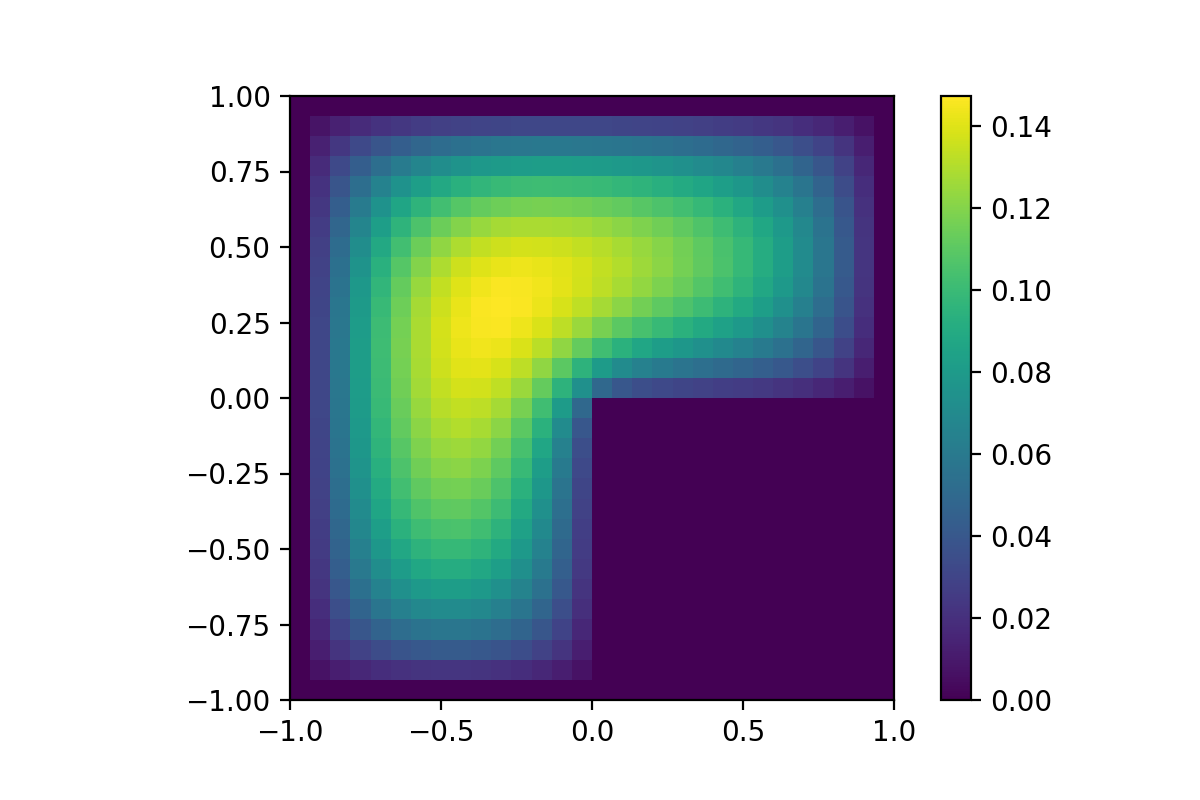
\includegraphics[width=4cm]{sol37.png}\\[2ex]
27 January 2020}
\author{Adéla Moravová \and Barbara Präg 
\vspace{-0.7cm}}


\begin{document}


\maketitle


\begin{frame}{Contents}
\tableofcontents
\end{frame}

\section{Poisson's equation}

\begin{frame}{Poisson's equation}

$\begin{cases}- \Delta u = f \ \text{in} \ \Omega  \\
\ \ \ \ \  u = 0 \ \text{on} \ \partial \Omega 
\end{cases}$\\[0.5cm] \pause

Weak formulation with solution $u\in H_0^1(\Omega)$:\\

$\displaystyle a(u,v) = \int_\Omega \nabla u \cdot \nabla v \ \text{d}x = \int_\Omega f v \ \text{d}x = (f,v) \ \ \ \forall v \in H_0^1(\Omega)$\\[0.5cm]

\pause

\begin{minipage}[t]{0.3\textwidth}
\centering
	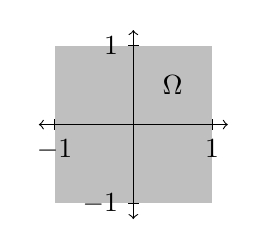
\begin{tikzpicture}[scale=1]
	%\draw (-1,-1) -- (-1,1) -- (1,1) -- (1,-1) -- (-1,-1);
 	\fill[fill = lightgray] (-1,-1) rectangle (1,1);

	\draw[<->] (-1.2,0) -- (1.2,0) coordinate (x axis);
 	\draw[<->] (0,-1.2) -- (0,1.2) coordinate (y axis);
 	
 	\foreach \x/\xtext in {-1/-1, 1/1}
 		\draw (\x,2pt) -- (\x,-2pt) node[anchor=north] {$\xtext$};
 	\foreach \y/\ytext in {-1/-1, 1/1}
 		\draw (2pt,\y) -- (-2pt,\y) node[anchor=east] {$\ytext$};
 		
 	\draw (0.5,0.5) node {$\Omega$};
 		
\end{tikzpicture}\\
\end{minipage}
\begin{minipage}[b]{0.3\textwidth}
\centering
	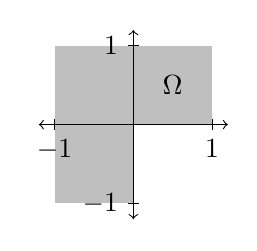
\begin{tikzpicture}[scale=1]
	%\draw (-1,-1) -- (-1,1) -- (1,1) -- (1,-1) -- (-1,-1);
 	\fill[fill = lightgray] (-1,-1) rectangle (1,1);
 	\fill[fill = white] (0,0) rectangle (1,-1);

	\draw[<->] (-1.2,0) -- (1.2,0) coordinate (x axis);
 	\draw[<->] (0,-1.2) -- (0,1.2) coordinate (y axis);
 	
 	\foreach \x/\xtext in {-1/-1, 1/1}
 		\draw (\x,2pt) -- (\x,-2pt) node[anchor=north] {$\xtext$};
 	\foreach \y/\ytext in {-1/-1, 1/1}
 		\draw (2pt,\y) -- (-2pt,\y) node[anchor=east] {$\ytext$};
 		
 	\draw (0.5,0.5) node {$\Omega$};
 		
\end{tikzpicture}
\end{minipage}
\begin{minipage}[b]{0.3\textwidth}
	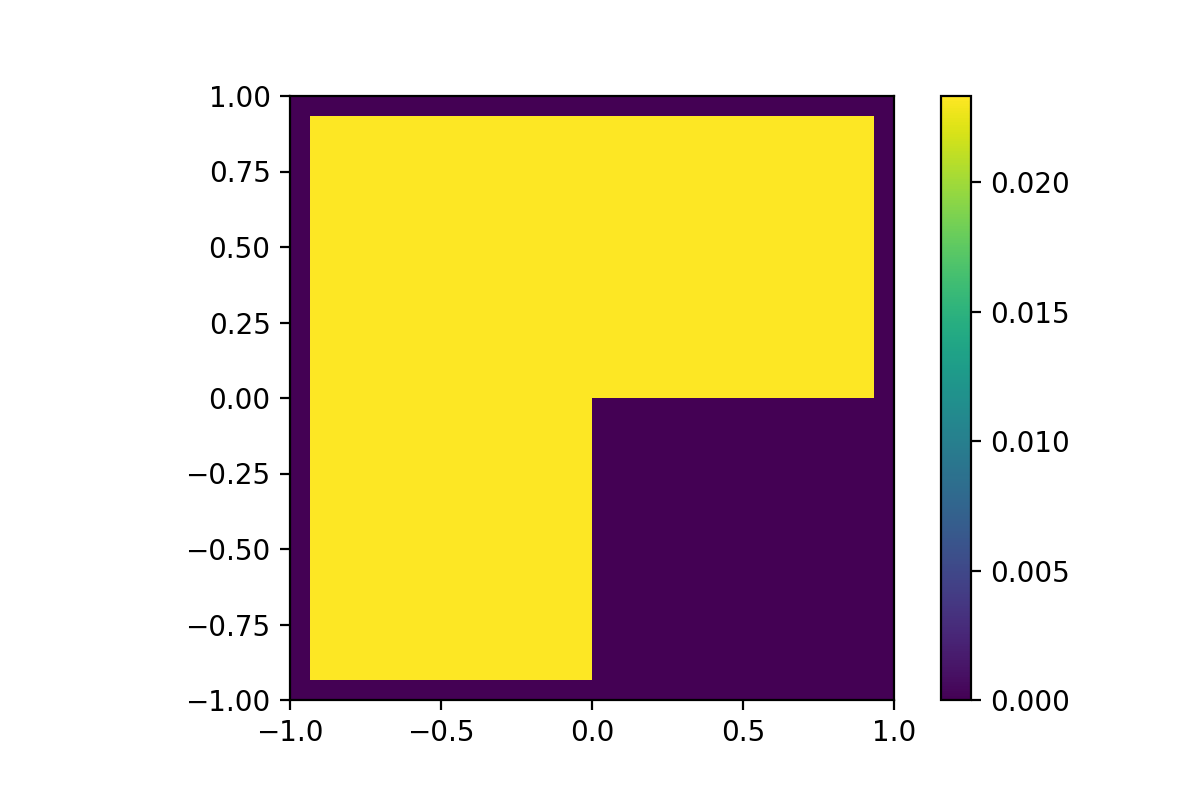
\includegraphics[height=2.6cm,trim=0 0 3.4cm 0,clip=true]{sol1.png}
\end{minipage}

\end{frame}


\begin{frame}{Reminder: Sobolev spaces and their norms}
Let $\Omega \subset \mathbb{R}^n$ be open.\\[0.8cm]
\pause
$\displaystyle H^k(\Omega) = \{u \in L^2(\Omega): D^\alpha u \in L^2(\Omega)$ for all $|\alpha| \leq k\}$\\[0.5cm]
%--> $H^0(\Omega) = L^2(\Omega)$
\pause
$\displaystyle (u,v)_{H^k} = \sum_{|\alpha| \leq k} \int_\Omega D^\alpha u \ D^\alpha v \ \text{d}x$\\[0.5cm]
\pause
$\displaystyle \|u\|_{H^k(\Omega)} = \sqrt{(u,u)_{H^k}}$\\[0.5cm]
\pause
$\displaystyle u \in H_0^1(\Omega)$ if $u \in H^1(\Omega)$ and "$u |_ { \partial \Omega} = 0$"
\end{frame}


\section{Shift theorems}

\begin{frame}{Shift theorems}
Let $\Omega$ be a \textbf{convex polygonal} domain in $\mathbb{R}^2$ and $u$ the weak solution to our problem. \pause Then 
\begin{equation*}
	\| u \|_{H^2} \leq C \| f \|_{H^0} \ \text{for} \ f \in H^0(\Omega) = L^2(\Omega).
\end{equation*}\\[1ex]
% --> The solution is two times more "regular" than the right-hand side f. The elliptic differential operator "smoothes"
\pause
\textbf{Fractional-order Sobolev spaces:}\\[0.1cm]
Let $0<s<1$.\\[0.2cm]
\pause

	$\displaystyle H^s(\Omega) = W^{s,2}(\Omega) := \left\{ u \in L^2(\Omega): \frac{|u(x)-u(y)|}{|x-y|^{1+s}} \in  L^2(\Omega \times \Omega) \right\}$

	$\displaystyle\|u\|_{H^s(\Omega)} := \left( \|u\|_{L^2(\Omega)}^2 + \iint_{\Omega \times \Omega} \left( \frac{|u(x)-u(y)|}{|x-y|^{1+s}} \right)^2 \ \text{d}x \ \text{d}y \right)^\frac{1}{2}$

\end{frame}


\begin{frame}{Shift theorems}

Let $0 < s < s_0 < 1$ ($s_0$ is a constant depending on the domain). Then,\vspace{-0.2cm}

\begin{equation*}
	\|u\|_{H^{2+s}} \leq C \|f\|_{H^s} \ \text{for} \ f \in H^s(\Omega).
\end{equation*}\\[0.5cm]

\pause
For a smooth boundary $\partial \Omega$ it even holds that \begin{equation*}
	\|u\|_{H^{m+2}} \leq C \|f\|_{H^m} \ \text{for} \ f \in  H^m(\Omega) \ \text{and} \ m \in \mathbb{N}_0.
\end{equation*}
\pause
Here, $m=0$ and $m=1$ also hold for a square domain.
%Do we need to include m=-1? Should we then define it?
%

%\textbf{But:} This regularity estimate never holds for  for non-convex polygonal domains like the L-shape.

% Similar result can be obtained for fractional-order Sobolev spaces.
% Add more here??
\end{frame}



\begin{frame}{Numerical solution of Poisson's equation on an L-shaped domain}

regular triangulation with right-angled triangles\\
finite element method\\
conjugate gradients solver\\

\animategraphics[autoresume, height=3.5cm]{8}{sol}{1}{15} \animategraphics[autoresume, height=4cm]{8}{gif}{0}{20}

\end{frame}



\begin{frame}{Regularity problem of the L}

\begin{minipage}{0.4\textwidth}
\begin{tikzpicture}
    \node[anchor=south west,inner sep=0] (image) at (0,0) {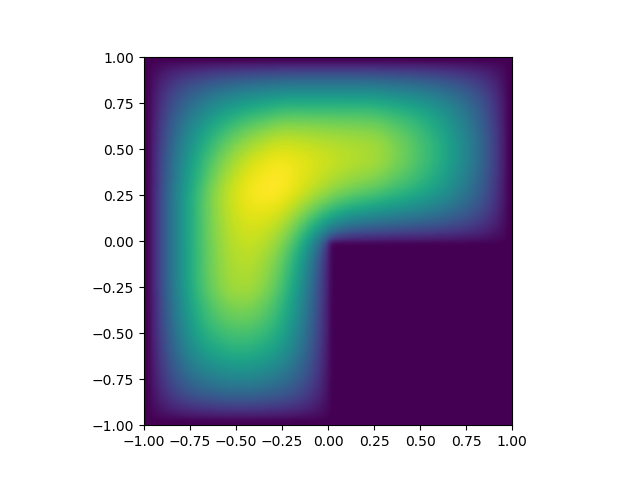
\includegraphics[height=4cm, trim=2cm 0 1.5cm 0, clip=true]{Figure_1.png}};
    \begin{scope}[x={(image.south east)},y={(image.north west)}]
    	\draw[->,red, ultra thick] (0.5,0.4845) -- (0.5,0.7);
    	\draw[->,red, ultra thick] (0.5,0.49) -- (0.3,0.49);
    	\draw[->,red, ultra thick] (0.5,0.49) -- (0.32,0.68);
        %\draw[red,ultra thick,rounded corners] (0.62,0.65) rectangle (0.78,0.75);
    \end{scope}
\end{tikzpicture}
\end{minipage}\pause
\begin{minipage}{0.5\textwidth}
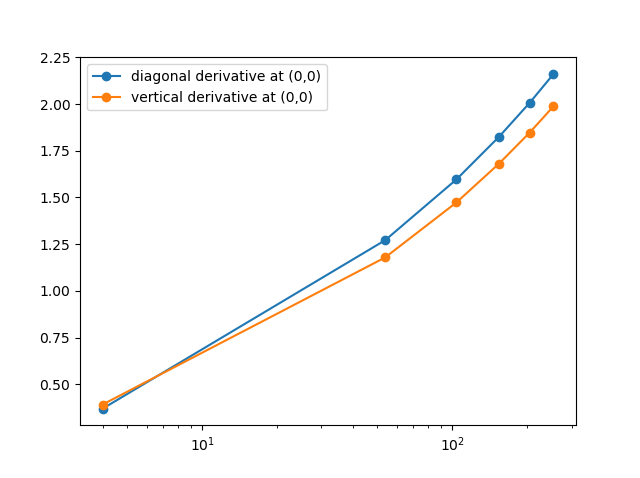
\includegraphics[height=5cm]{derivatives2.png}
\end{minipage}

\end{frame}



\section{Finite element error}

\begin{frame}{Finite element error}
Let $u$ be the weak solution of our elliptic problem,\\
$\mathcal{T}_h$ a regular triangulation of a polygonal domain $\Omega$, $V_h = \{u \in C(\Omega) \cap H_0^1(\Omega): u|_T = \mathbb{P}^1 \ \forall\ T \in \mathcal{T}_h \}$ a piecewise linear finite element space and $u_h \in V_h$ the finite element solution, i.e., $ u_h \in V_h$ such that $a(u_h,v_h) = (f,v_h)$ for all $v_h \in V_h$.\\[0.3cm]
\pause
Then,
% i.e., $ u_h \in V_h$ such that $a(u_h,v_h) = (f,v_h)$ for all $v_h \in V_h$,
\begin{equation*}
	\|u - u_h\|_{H^1} \leq C h \|u\|_{H^2}. 
\end{equation*}	
	
%Under the assumption that , we also get an $L^2$ estimation for the finite element error:\\[1ex]

\end{frame}



\begin{frame}{Finite element error}
Additionally, assume that $\Omega$ is convex and the shift theorem $\| u \|_{H^2} \leq C \| f \|_{H^0}$ holds.\\[0.1cm]
\pause
Let $z \in H_0^1(\Omega)$ be a solution of $a(z,v) = (u-u_h,v), \ v \in H_0^1(\Omega)$.\\[0.1cm]
\pause
For all $z_h \in V_h \subset H_0^1(\Omega)$: $a(u,z_h) = (f,z_h) = a(u_h,z_h)$.\\ \pause
$\Rightarrow a(u-u_h,z_h) = 0$.\\
% $u-u_h \in H_0^1(\Omega)$, cf. \ref{fee}. and \ref{st}???
\pause
\begin{align*}
\|u-u_h\|_{L^2}^2 &= \visible<6->{(u-u_h,u-u_h) =}\\
&\visible<7->{= a(z,u-u_h) =} \visible<8->{a(z-z_h,u-u_h) \leq}\\
&\visible<9->{\leq \|\nabla(u-u_h)\|_{L^2} \cdot \|\nabla(z-z_h)\|_{L^2} \leq}\\
&\visible<10->{\leq \|u-u_h\|_{H^1}  \cdot \|z-z_h\|_{H^1} \leq}\\
\visible<11>{&\leq Ch^2 \cdot \|u\|_{H^2} \cdot \|z\|_{H^2} \leq}\\
\end{align*}

\end{frame}

\begin{frame}{Finite element error}
\begin{align*}
&\leq \tilde{C}h^2\cdot \|u\|_{H^2} \cdot \|u-u_h\|_{H^0} =\\
&\visible<2->{= \tilde{C}h^2\cdot \|u\|_{H^2}\cdot \|u-u_h\|_{L^2}.}
\end{align*}\\

\pause
\pause

\medskip
$\Rightarrow \|u-u_h\|_{L^2}^2 \leq \tilde{C}h^2\cdot \|u\|_{H^2}\cdot \|u-u_h\|_{L^2}$ \pause
$\Rightarrow \|u-u_h\|_{L^2} \leq \tilde{C}h^2 \cdot \|u\|_{H^2}$.\\[2.5ex]

\pause
If $\Omega$ is not convex, this inequality need not hold true, too.\\[0.9cm]
\end{frame}


\begin{frame}{Comparison of convergence rates}

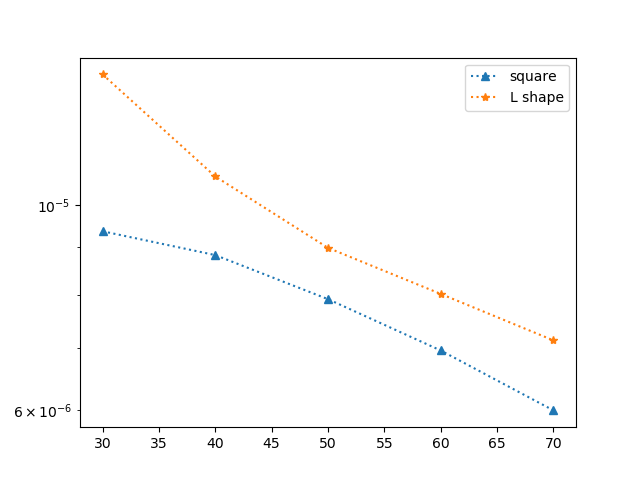
\includegraphics[scale =0.5 \textwidth]{convergence_rate_after_n_steps.png} 
\end{frame}


\section{Refining the grid}

\begin{frame}{Refining the grid}

\centering
\begin{minipage}{0.4\textwidth}
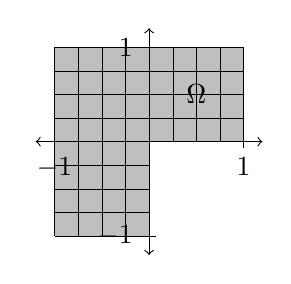
\begin{tikzpicture}[scale=1.2]
	%\draw (-1,-1) -- (-1,1) -- (1,1) -- (1,-1) -- (-1,-1);
 	\fill[fill = lightgray] (-1,-1) rectangle (1,1);
 	\draw[step=0.25cm, ultra thin] (-1,-1) grid (1,1);
	\fill[fill = white] (0,0) rectangle (1.1,-1.1);

	\draw[<->] (-1.2,0) -- (1.2,0) coordinate (x axis);
 	\draw[<->] (0,-1.2) -- (0,1.2) coordinate (y axis);
 	
 	\foreach \x/\xtext in {-1/-1, 1/1}
 		\draw (\x,2pt) -- (\x,-2pt) node[anchor=north] {$\xtext$};
 	\foreach \y/\ytext in {-1/-1, 1/1}
 		\draw (2pt,\y) -- (-2pt,\y) node[anchor=east] {$\ytext$};
 		
 	\draw (0.5,0.5) node {$\Omega$};
 		
\end{tikzpicture}

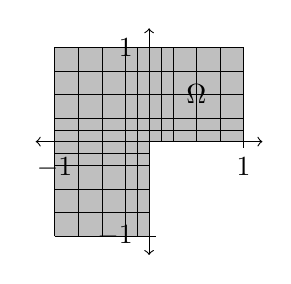
\begin{tikzpicture}[scale=1.2]
	%\draw (-1,-1) -- (-1,1) -- (1,1) -- (1,-1) -- (-1,-1);
 	\fill[fill = lightgray] (-1,-1) rectangle (1,1);
 	\draw[step=0.25cm, ultra thin] (-1,-1) grid (1,1);
 	\foreach \x in {0.125,-0.125}
 		\draw[ultra thin] (\x,1) -- (\x,-1);
 	\foreach \y in {0.125,-0.125}
 		\draw[ultra thin] (1,\y) -- (-1,\y);

 	\fill[fill = white] (0,0) rectangle (1.1,-1.1);

	\draw[<->] (-1.2,0) -- (1.2,0) coordinate (x axis);
 	\draw[<->] (0,-1.2) -- (0,1.2) coordinate (y axis);
 	
 	\foreach \x/\xtext in {-1/-1, 1/1}
 		\draw (\x,2pt) -- (\x,-2pt) node[anchor=north] {$\xtext$};
 	\foreach \y/\ytext in {-1/-1, 1/1}
 		\draw (2pt,\y) -- (-2pt,\y) node[anchor=east] {$\ytext$};
 		
 	\draw (0.5,0.5) node {$\Omega$};
 		
\end{tikzpicture}
\end{minipage}
\begin{minipage}{0.5\textwidth}
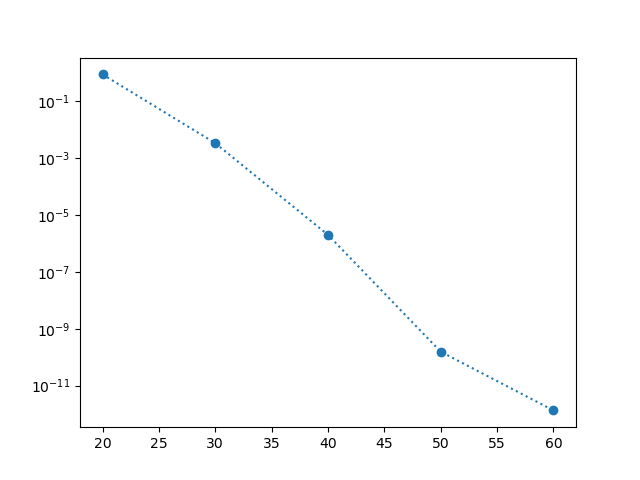
\includegraphics[scale=0.7\textwidth]{adapted.png}
\end{minipage}
\end{frame}




\begin{frame}
\vfill

\centering \Large{\textbf{Thank you for your attention!}}\\[10ex]

\begin{figure}[b!]
\normalsize
\flushleft
\vfill
\small
\textbf{Literature:} \\
Demlow, Alan: \emph{Notes for Math 663. Chapter 1.} Spring 2016.\\
Bacuta, C., Bramble, J. H., Xu, Jinchao: \emph{Regularity estimates for elliptic boundary value problems with smooth data on polygonal domains.} January 8, 2003.
\end{figure}
\end{frame}



\end{document}
